\begin{figure}[t]
\centering
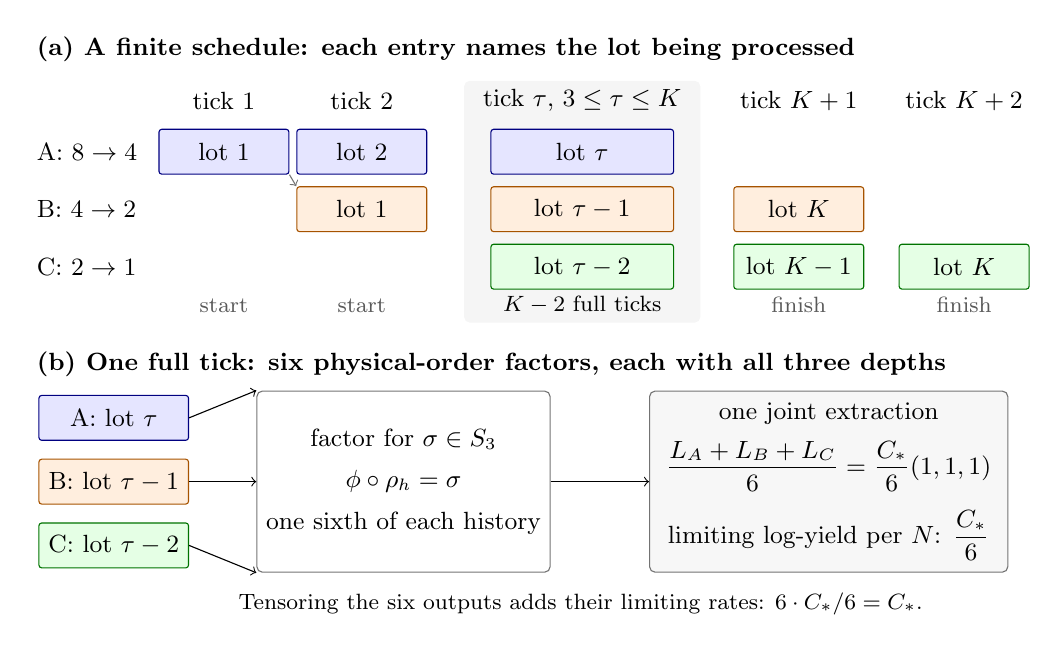
\begin{tikzpicture}[x=1cm,y=1cm,font=\small,
  stageA/.style={fill=blue!10,draw=blue!50!black},
  stageB/.style={fill=orange!13,draw=orange!65!black},
  stageC/.style={fill=green!10,draw=green!45!black},
  cell/.style={minimum height=.57cm,minimum width=1.65cm,
               rounded corners=1pt,inner sep=3pt,align=center}]
\node[anchor=west,font=\bfseries\small] at (0,0.65)
  {(a) A finite schedule: each entry names the lot being processed};
\fill[black!4,rounded corners=2pt] (5.55,-2.82) rectangle (8.55,0.25);
\node at (2.50,0) {tick $1$};
\node at (4.25,0) {tick $2$};
\node[align=center] at (7.05,0) {tick $\tau$, $3\leq\tau\leq K$};
\node at (9.80,0) {tick $K+1$};
\node at (11.90,0) {tick $K+2$};
\node[anchor=west] at (0,-.65) {A: $8\to4$};
\node[anchor=west] at (0,-1.38) {B: $4\to2$};
\node[anchor=west] at (0,-2.11) {C: $2\to1$};
\node[cell,stageA] (a1) at (2.50,-.65) {lot $1$};
\node[cell,stageA] at (4.25,-.65) {lot $2$};
\node[cell,stageA,minimum width=2.32cm] at (7.05,-.65) {lot $\tau$};
\node[cell,stageB] (b1) at (4.25,-1.38) {lot $1$};
\node[cell,stageB,minimum width=2.32cm] at (7.05,-1.38) {lot $\tau-1$};
\node[cell,stageB] at (9.80,-1.38) {lot $K$};
\node[cell,stageC,minimum width=2.32cm] (cfull) at (7.05,-2.11) {lot $\tau-2$};
\node[cell,stageC] at (9.80,-2.11) {lot $K-1$};
\node[cell,stageC] at (11.90,-2.11) {lot $K$};
\draw[->,thin,black!55] (a1.south east) -- (b1.north west);
\node[font=\footnotesize,black!65] at (2.50,-2.60) {start};
\node[font=\footnotesize,black!65] at (4.25,-2.60) {start};
\node[font=\footnotesize] at (7.05,-2.60) {$K-2$ full ticks};
\node[font=\footnotesize,black!65] at (9.80,-2.60) {finish};
\node[font=\footnotesize,black!65] at (11.90,-2.60) {finish};

\node[anchor=west,font=\bfseries\small] at (0,-3.35)
 {(b) One full tick: six physical-order factors, each with all three depths};
\node[cell,stageA,minimum width=1.90cm] (aa) at (1.10,-4.03)
 {A: lot $\tau$};
\node[cell,stageB,minimum width=1.90cm] (bb) at (1.10,-4.84)
 {B: lot $\tau-1$};
\node[cell,stageC,minimum width=1.90cm] (cc) at (1.10,-5.65)
 {C: lot $\tau-2$};
\node[draw=black!55,rounded corners=2pt,align=center,
      minimum width=3.12cm,minimum height=2.30cm] (order)
 at (4.78,-4.84)
 {factor for $\sigma\in S_3$\\[4pt]
  $\phi\circ\rho_h=\sigma$\\[4pt]
  one sixth of each history};
\draw[->] (aa.east) -- (order.north west);
\draw[->] (bb.east) -- (order.west);
\draw[->] (cc.east) -- (order.south west);
\node[draw=black!55,fill=black!3,rounded corners=2pt,align=center,
      minimum width=4.55cm,minimum height=2.30cm] (joint)
 at (10.18,-4.84)
 {one joint extraction\\[5pt]
  $\displaystyle\frac{L_A+L_B+L_C}{6}
      =\frac{C_*}{6}(1,1,1)$\\[6pt]
  limiting log-yield per $N$: $\displaystyle\frac{C_*}{6}$};
\draw[->] (order.east) -- (joint.west);
\node[align=center,font=\footnotesize] at (7.03,-6.39)
 {Tensoring the six outputs adds their limiting rates: $6\cdot C_*/6=C_*$.};
\end{tikzpicture}
\caption{Mixed-depth extraction with finite boundaries ($K\geq2$).
A lot advances one stage per tick, while a full tick combines three
different lots.  Within each physical-order factor, the common order
$\sigma$ permits one application of Theorem~\ref{thm:joint-step} to
the summed capacities.  The four boundary ticks have the positive
minima appearing in \eqref{eq:boundary-deficit}; they incur only the
fixed deficit $\beta$.  The middle column is absent when $K=2$.}
\label{fig:pipeline}
\end{figure}
